\section{Related work}
\label{sec:related}

\paragraph{Deep generative models of 3D shapes.}
Multiple 3D shape representations have been used in the context of
deep generative models.
3D voxel grids~\cite{choy20163d, prgan} are a natural extension to image-based architectures,
but suffer from high memory footprint requirements.
Sparse occupancy grids~\cite{Wang-2017-ocnn, tatarchenko2017octree, hie3dcnn, matryoshka} alleviate this issue using a hierarchical grid,
but they are still not able to generate detailed shapes and they require additional bookkeeping.
Multi-view representations ~\cite{Soltani17, LunGKMW17}, point clouds~\cite{fan2016point, mrt18, pcagan, latentpc}, mesh deformations~\cite{pixel2mesh, cmrKanazawa18}
and implicit functions~\cite{park2019deepsdf, mescheder2019occupancy, chen2019learning, genova2019learning} provide alternatives that are compact and capable
of generating detailed shapes.
However, these approaches are focused on reconstructing accurate 3D shapes and
are not amenable to tasks like editing.
Our goal is different: we explore generative models to produce sets of handles --
summarized shape representations that can be easily manipulated by users.

\begin{figure}
\centering
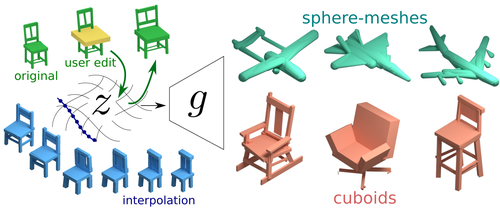
\includegraphics[width=0.8\linewidth]{handles/imgs/pipeline.png}
\caption{\label{fig:handles}
\textbf{Overview}.
We propose a method to train a generative model $g$ for sets of shape handles.
Once trained, the latent representation $z$ can also be used in applications like
shape editing and interpolation.}
\vspace{-14pt}
\end{figure}


%Even though images require a smaller memory footprint than occupancy grids,
%they are not ideal either: as there is no explicit 3D representation, some synthesized pixels do not correspond to any surface, while others may appear in many different views but with no consensus on the corresponding 3D point, leading to a sub-optimal representation.
%Meshes and point clouds do not suffer from these limitations.
%Every generated triangle or point is, by construction, a part of the surface.
%However, meshes are notoriously hard to generate using deep neural networks.
%The techniques are usually limited to generating vertex positions in a pre-defined mesh topology~\cite{},
%or by generating meshes as a post-processing step~\cite{}.
%On the other hand, point cloud generation techniques are more flexible, capable of approximating
%shapes of arbitrary topology.
%While some methods generate 3D point clouds directly~\cite{}, others generate points via learned surface parameterizations~\cite{}.
%A key component of these approaches is the utilization of permutation invariant losses capable
%of computing similarity between sets of points.
%In this work, we extend these losses to allow comparisons between sets of primitives.
%
%Recent research focuses on representing shapes as the level sets of implicit
%functions parameterized by neural networks~\cite{}.
%This representation is capable of seamlessly representing shapes of different topologies
%with low memory footprints.
%However, implicit functions are high dimensional %and often non-parsimonious \nathan{ I am not sure this can be argued that implicit forms imply non-parsimony it depends how they are used.  } \rui{this is a well-known term?} 
%and are not naturally suitable
%for shape editing or other high-level reasoning tasks, like path planning or grasping.
%Our goal is to generate shapes represented by a small set of primitive components
%that can be easily manipulated and utilized by high-level reasoning systems.  \rui{the above two paragraphs are very long and it could be dramatically simplified, by saying that these techniques are focused on generating detailed 3D shapes but they are not naturally amenable for shape editing. Our goal is different, blah blah.}

Two closely related methods to ours are Tulsiani et al.~\cite{Tulsiani2017} and Paschalidou et al.~\cite{Paschalidou2019} where they propose models
to generate shapes as a collection of primitives \emph{without supervision}.
%The problem we tackle here is fundamentally different -- 
In contrast, we are focused
on creating models capable of utilizing shape decompositions provided by external
agents; either a human annotator or a shape summarization technique.
We demonstrate that, by using the extra information provided by annotations or well known
geometric processing techniques, our method is capable of generating
more accurate shapes while keeping the representation interpretable and intuitive for easy
editing.
Other approaches focused on learning shape structures through stronger 
supervision~\cite{li_sig17, mo2019structurenet, im2struct}, requiring not only handle description,
but also relationships between them, e.g. support, symmetry, adjacency, hierarchy, etc.
In contrast, our method models shapes as sets and we show that inter-handle relationships
can be learned directly from data, so that the latent space induced by our model can be used to guide shape editing, completion, and interpolation tasks.
Furthermore, we present a general framework that can be easily adapted to different types of handles,
not only a single parametric family, like cuboids~\cite{Tulsiani2017, mo2019structurenet, li_sig17} or superquadrics~\cite{Paschalidou2019}.

\paragraph{Methods for shape decomposition.}
Shape decomposition has been extensively studied by the geometry processing
literature. The task is to approximate a complex shape as a set of simpler, lower-dimensional
parts that are amenable for editing. We refer to these parts as \emph{shape handles}. Early cognitive studies have shown that humans tend to reason about 3D shapes as a union
of convex components~\cite{partsrecognition}. Multiple approaches have explored decomposing shapes in this manner~\cite{acd, minimumncd, acanalysis}.
However, those approaches are likely to generate too many parts, making them difficult to manipulate.
This problem was addressed by later shape approximation methods such as cages~\cite{obbcage}, 3D curves~\cite{gsmc_iwires_sig_09,mzlsgm_abstraction_siga_09,Gori2017}
and sphere-meshes~\cite{spheremesh}, which are shown very useful in shape editing and other high-level tasks. Our method is flexible to work with various types of shape handles, and in particular we show experiments using cuboids as well as sphere-meshes.
%but have not been applied in deep generative models.
%Our model can easily work with different types of handles, such as cuboids and sphere-meshes. 
%, a generalization of regular triangle meshes where each vertex also
%has a radius parameter. Here each triangle represents the interpolation of the spheres located at each vertex.
%They have been applied to shape deformation~\cite{spheremesh}, tracking~\cite{smhandtrack} and
%animation~\cite{animatedsm}.
%In particular, we use the sphere-mesh computation procedure presented in~\cite{} to
%generate training data for our model.
%Then, we demonstrate how our model can be used in various shape generative tasks using
%sphere-mesh representations.

Several closely related methods to ours approximate complex shapes using
primitives such as cylinders~\cite{gdc} or cuboids~\cite{obbcage}.
These approximations are easy to interpret and manipulate
by humans. However, most existing methods rely solely on geometric cues for computing primitives, which
can lead to counter-intuitive decompositions.
In contrast, our method takes supervision from semantic information provided
by human annotators or shape summarization techniques, 
and therefore our results more accurately match human intuition. 
%\rui{do we want to add something about editing in latent space?}
%Specifically, we leverage fine-grained part segmentations from Partnet~\cite{partnet} as
%primitives and use them as training data for our model. 
%if we have a model capable of generating shapes represented by a set of shape handles,
%we are able to leverage fine-grained part segmentations from a dataset~\cite{} as
%primitives and use them as training data for in our model.
%The result is a network that decomposes the shapes following the clues provided by human
%annotators, which leads to more intuitive approximations.% than prior unsupervised methods.


